

\section{Data Understanding}\label{chap:dataUnderstanding}
This stage of the CRISP-DM process focuses on initial data analysis to understand the structure, content, and quality of the data provided for the project. This involves collecting, describing, exploring, and assessing the quality of the data in order to ensure it is suitable for modeling.

\subsection{Initial data collection }\label{sec:initialDataCollection}
For our analysis, we utilized historical data from an existing rental and hotel aggregator platform. The dataset spans several years and covers multiple seasonal periods. It includes both information about rental listings and their respective hosts.

The main data sources was CSV file with rental offer information exported from the aggregator (covering three years (2018--2020)). The dataset is available on \href{https://www.kaggle.com/datasets/hazujaf/airbnb-price-prediction-in-rio-de-janeiro-python?resource=download}{Kaggle}\cite{airbnb_rio_kaggle}, which originally compiled publicly available information from the Airbnb website for Rio de Janeiro.

\subsection{Data Description }\label{sec:dataDescription}
Our data contains about 784K records and 108 different attributes. The entire dataset weighs about 2.5 GB.
Among the features we have:
\begin{itemize}
    \item \textbf{geodata} --- housing position in coordinates
    \item \textbf{rental housing attributes} --- attributes that housing has (e.g., Wi-Fi, TV, number of beds, etc.)
    \item \textbf{host characteristics} --- host-related information
    \item \textbf{price} --- the price of housing
    \item \textbf{review score rating} --- historical rating on the aggregator platform
\end{itemize}

It is the review score rating that we want to learn how to predict in order to solve the cold start problem.

Overall, the structure and coverage of the data arc aligned with the project's goals, though some preprocessing and cleaning steps are necessary.

\subsection{Data Exploration\textit{[Core]}}\label{sec:dataExploration}

During this stage, we explored key aspects of the dataset through HQL queries and visual analysis. The goal was to identify trends, anomalies, and relationships that could guide future modeling efforts and transformations. Below we present the insights gained from our initial data mining queries.

\subsubsection*{1. Price and Rating Distribution in Popular Neighborhoods}

To understand pricing and quality dynamics across the most active regions, we selected the top 10 most frequently occurring neighborhoods with non-null entries. For these, we extracted corresponding price and review score ratings.

\vspace{0.5em}
\paragraph{Key insights}
\begin{itemize}
    \item Weak Correlation inside neighborhoods: High prices in neighborhoods do not guarantee top reviews in it. Leblon, as most expensive, ranks 7th in mean scores, while Flamengo which is cheaper, scores 4th highest in ratings.
    \item High-Value Opportunities: Flamengo and Laranjeiras combine low prices with top-tier scores, so can be considered as best neighborhoods to budget-conscious travelers.
    \item Price-Score Variability: large gaps between mean and median in prices suggest existence of small number of `luxury' offers, while gaps in scores - that there are small number of offers with small ratings
\end{itemize}

\vspace{1em}
\begin{figure}[H]
    \centering
    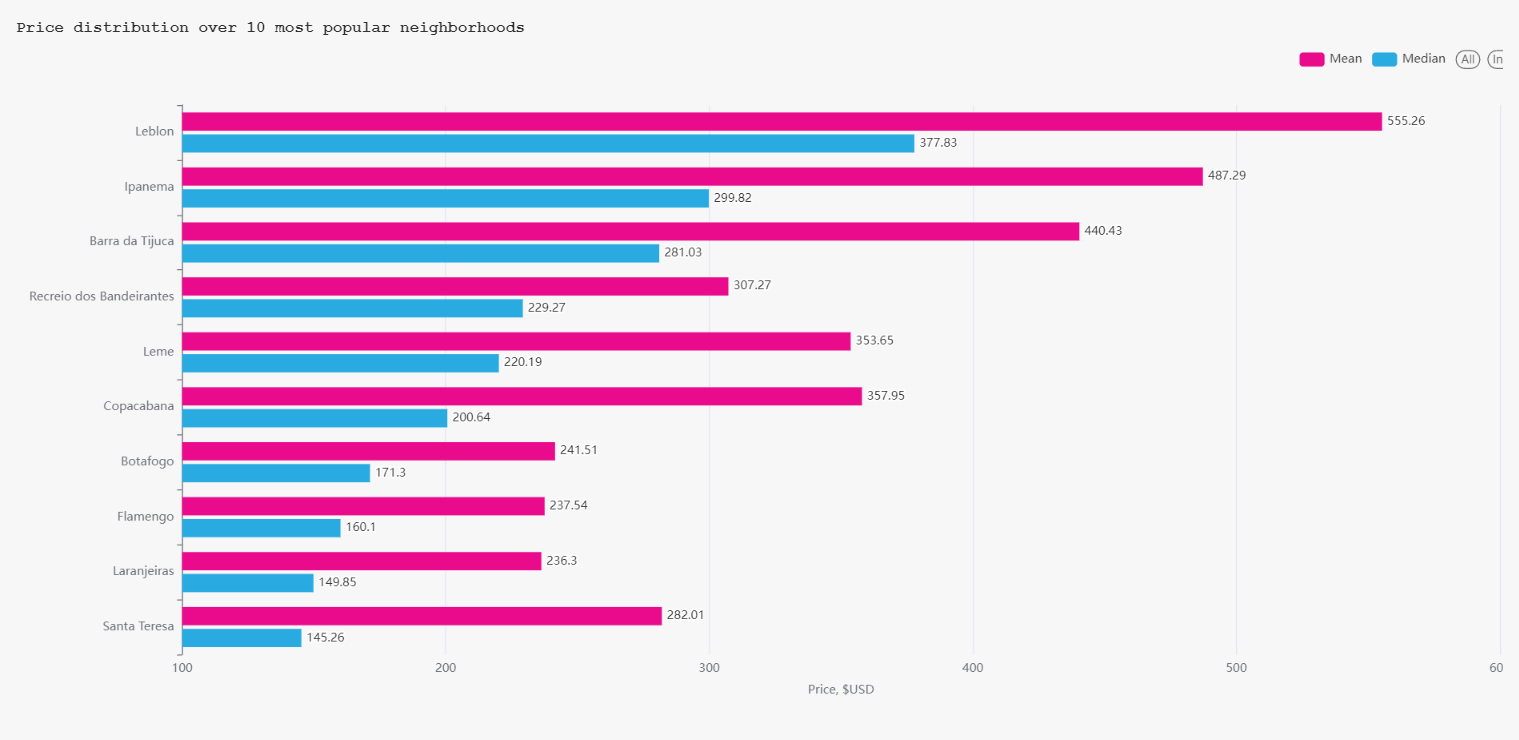
\includegraphics[width=1\textwidth]{images/q1_1.jpg}
    \caption{Price distribution over 10 most popular neighborhoods}\label{fig:figureq1}
\end{figure}

\vspace{1em}
\begin{figure}[H]
    \centering
    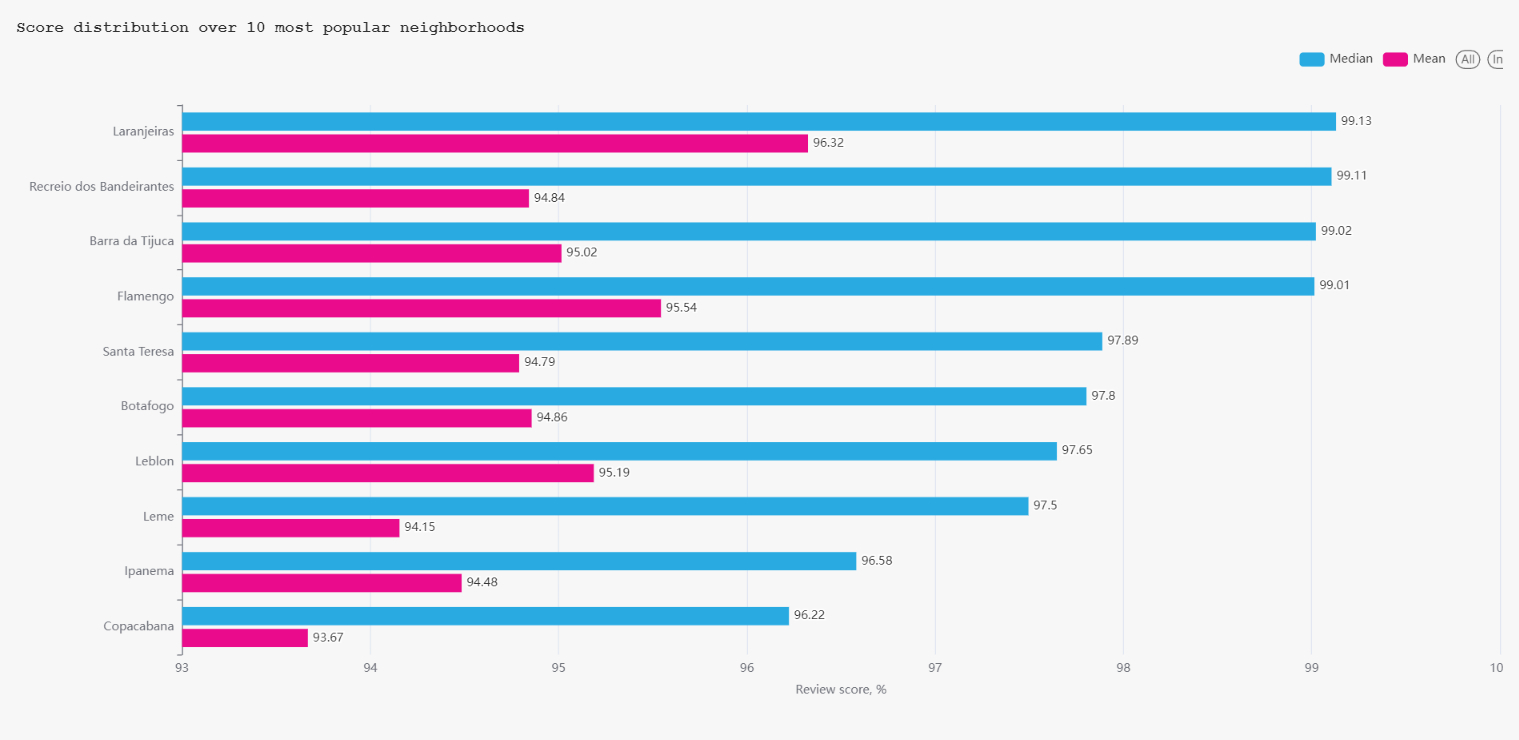
\includegraphics[width=1\textwidth]{images/q1_2.jpg}
    \caption{Score distribution over 10 most popular neighborhoods}\label{fig:figureq2}
\end{figure}

\subsubsection*{2. Relationship Between Night Limits, Pricing Buckets, and Ratings }

This section explores how booking restrictions (minimum/maximum nights), pricing tiers, and cancellation policies relate to review scores. Prices were bucketed into five meaningful intervals for better interpretability.

\vspace{0.5em}
\paragraph{Key insights}
\begin{itemize}
    \item Higher Prices, Generally Higher Scores (Across Policies): For most cancellation policies, the most expensive listings (2000+ dollars) tend to have the highest review scores. This suggests that price often correlates with quality/amenities that drive satisfaction, somewhat independently of the cancellation policy itself.
    \item Super Strict Policies loose: \texttt{super\_strict\_30} and \texttt{super\_strict\_60} tend to have scores lower than \texttt{moderate} or \texttt{flexible,} particularly for budget listings. This is a key finding --- a very strict policy on a mid-priced item might be perceived negatively.
    \item Moderate Policies Perform Well: \texttt{moderate} and \texttt{strict\_14\_with\_grace\_period} policies, particularly for listings priced 1000--1999\$ and 2000\$+, show very high average scores (often above 95.5\%--96\%). \texttt{Flexible} also performs strongly across price bands.
    \item Price Correlates with a Stay Length: there is a clear trend: as the price of the listing increases, both the typical minimum and maximum number of booking nights also tend to increase.
    \item Review Score with a Stay Length: another clear trend is that as the stay length of the listing increases, mean review score also increases. Also, there is a noticeable `phase transition' between 100--499\$ and 500--999\$ clusters: mean review score has here drastic increase.
\end{itemize}

\vspace{1em}
\begin{figure}[H]
    \centering
    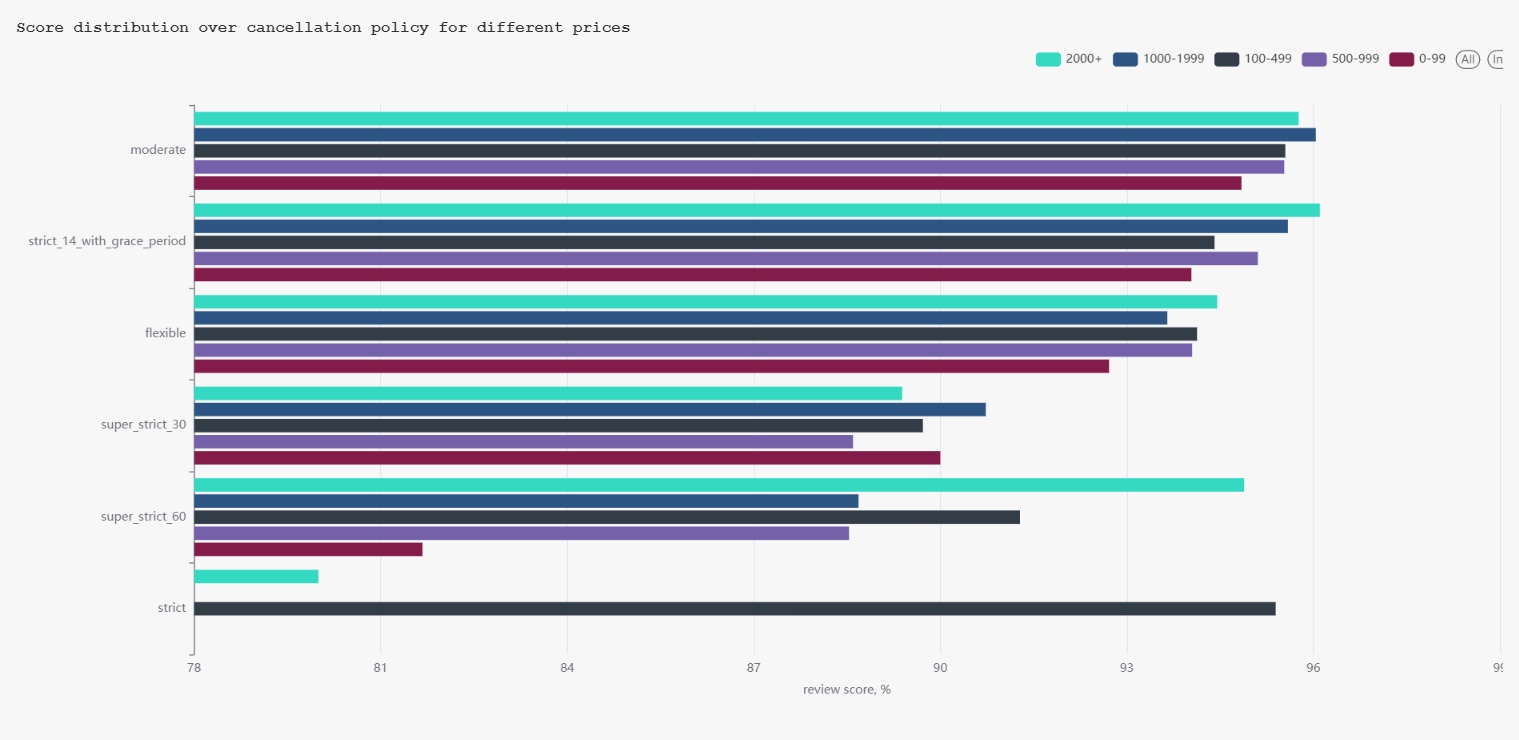
\includegraphics[width=1\textwidth]{images/q2_1.jpg}
    \caption{Score distribution over cancellation policy for different prices}\label{fig:figureq3}
\end{figure}

\vspace{1em}
\begin{figure}[H]
    \centering
    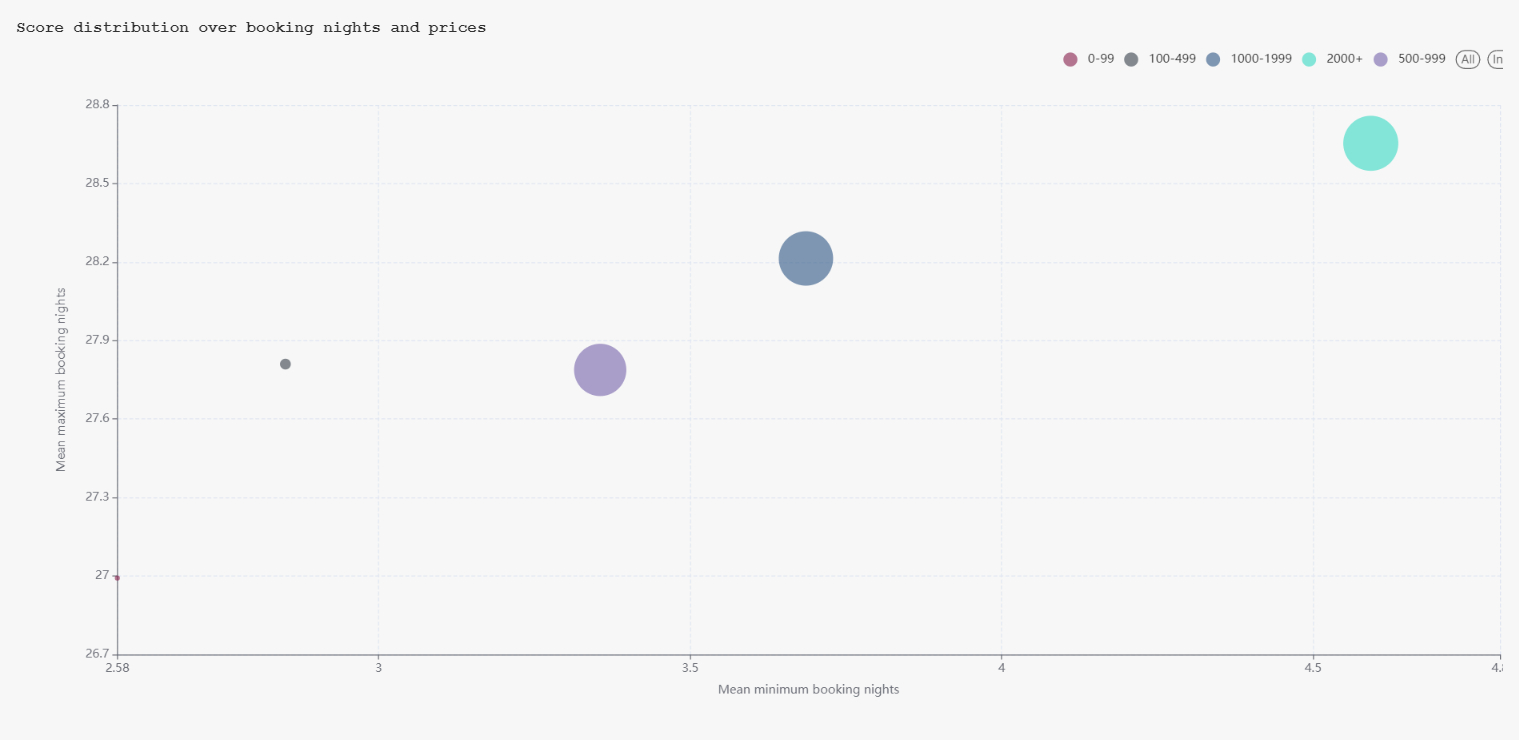
\includegraphics[width=1\textwidth]{images/q2_2.jpg}
    \caption{Score distribution over booking nights and prices}\label{fig:figureq4}
\end{figure}

\subsubsection*{3. Host Verification Features and Their Impact}

Here we examine how different host verification combinations affect guest ratings and pricing. Hosts were grouped into categories based on features like profile picture, identity verification, and superhost status.

\vspace{0.5em}
\paragraph{Key insights}
\begin{itemize}
    \item Superhosts alone achieve the highest review scores, even outperforming fully-featured hosts, suggesting that hosting experience across multiple listings correlates strongly with guest ratings.
    \item Adding verification on top of a profile picture (picture\_verified) slightly reduces the average score, which may indicate diminishing returns or that verification alone is not a strong trust signal.
    \item Listings with no host features have significantly lower scores, highlighting the risk of promoting anonymous or minimally detailed hosts.
    \item Interestingly, fully\_featured hosts (with all three attributes) do not significantly outperform hosts with just a picture or superhost status
\end{itemize}

\vspace{1em}
\begin{figure}[H]
    \centering
    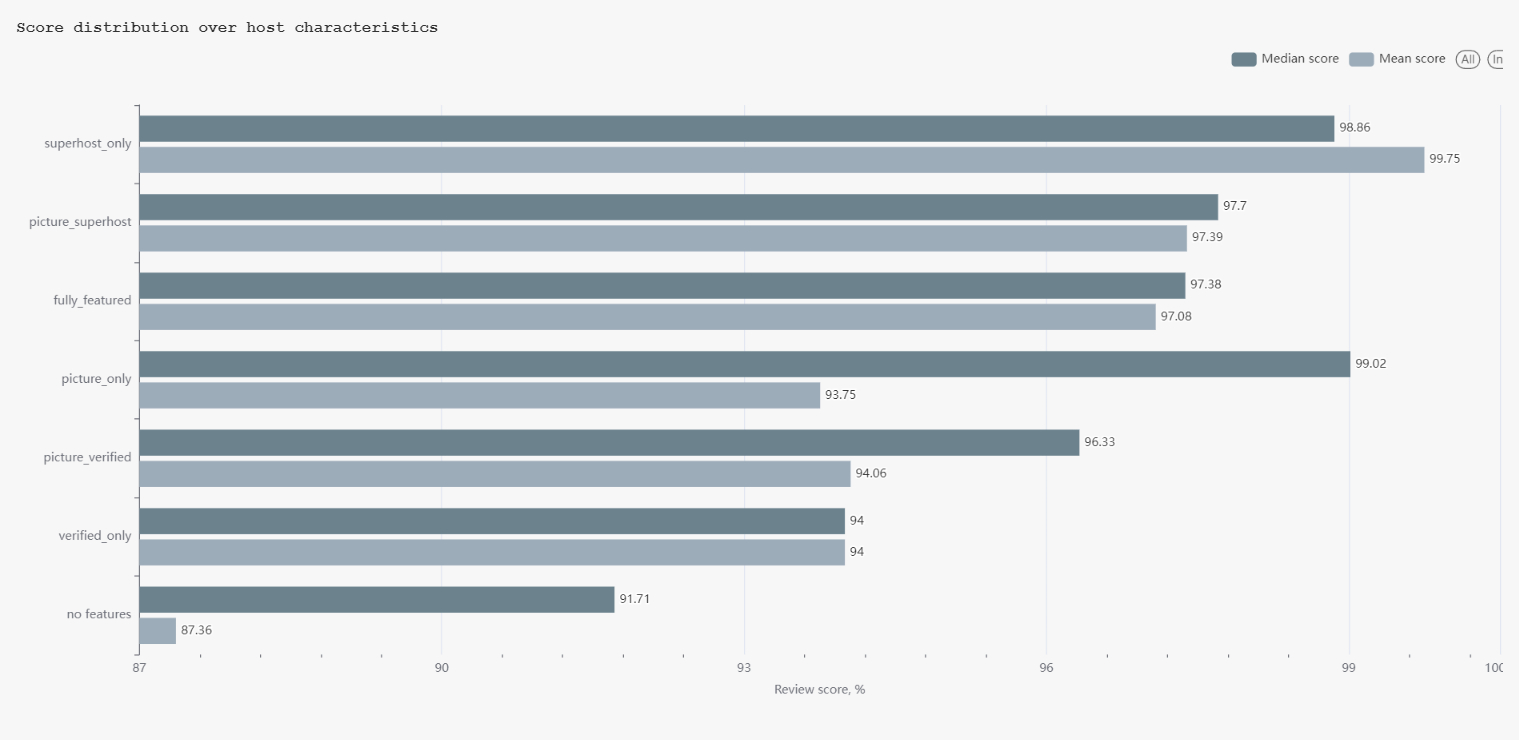
\includegraphics[width=1\textwidth]{images/q3_1.jpg}
    \caption{Score distribution over host characteristics}\label{fig:figureq4}
\end{figure}
\subsubsection*{Overall Findings and Impact}

These initial analyses provided several useful directions:
\begin{itemize}
    \item Identified key variables influencing pricing and satisfaction.
    \item Helped define valuable subpopulations (e.g., fully verified hosts).
    \item Offered a data-driven basis for later feature engineering and model design.
\end{itemize}

\subsubsection*{4. Popular Property and Room Type Analysis Over Time (Query 4)}

This query focuses on the top 10 property types and their associated room types. It tracks the price and review score ratings across months for combinations that are either:
\begin{itemize}
    \item Among the most common property types
    \item Among the most common property-room type pairs
\end{itemize}

Additionally, we construct a descriptive label combining room type and property type for intuitive grouping.

\vspace{0.5em}
\paragraph{Key insights}
\begin{itemize}
    \item Property Type Matters for Scores: for example,`Guest suite',`Loft' and`Townhouse' consistently achieve the highest review scores.
    \item Room Type is a Major Driver of Scores: while`Private room' consistently receives the highest scores, the`Shared room' and`Hotel room' receive significantly lower review scores.
    \item Winning Combinations for High Scores: combinations`Private room in Condominium' and`Private room in Apartment' consistently yields exceptionally higher scores.
    \item Price and Score Relationship: the most expensive popular options are typically`Entire home/apt' in House and in Apartment. While they score well, they don't consistently outperform the`Private room in Condominium/Apartment' in terms of guest scores. This suggests that while guests are willing to pay more for entire spaces, the quality in well-managed private rooms within desirable property types can lead to even higher scores.
    \item Seasonality Impact on Prices: prices for popular combinations show slight seasonal fluctuations. Prices during local fall and winter are slightly higher.

\end{itemize}

\vspace{1em}
\begin{figure}[H]
    \centering
    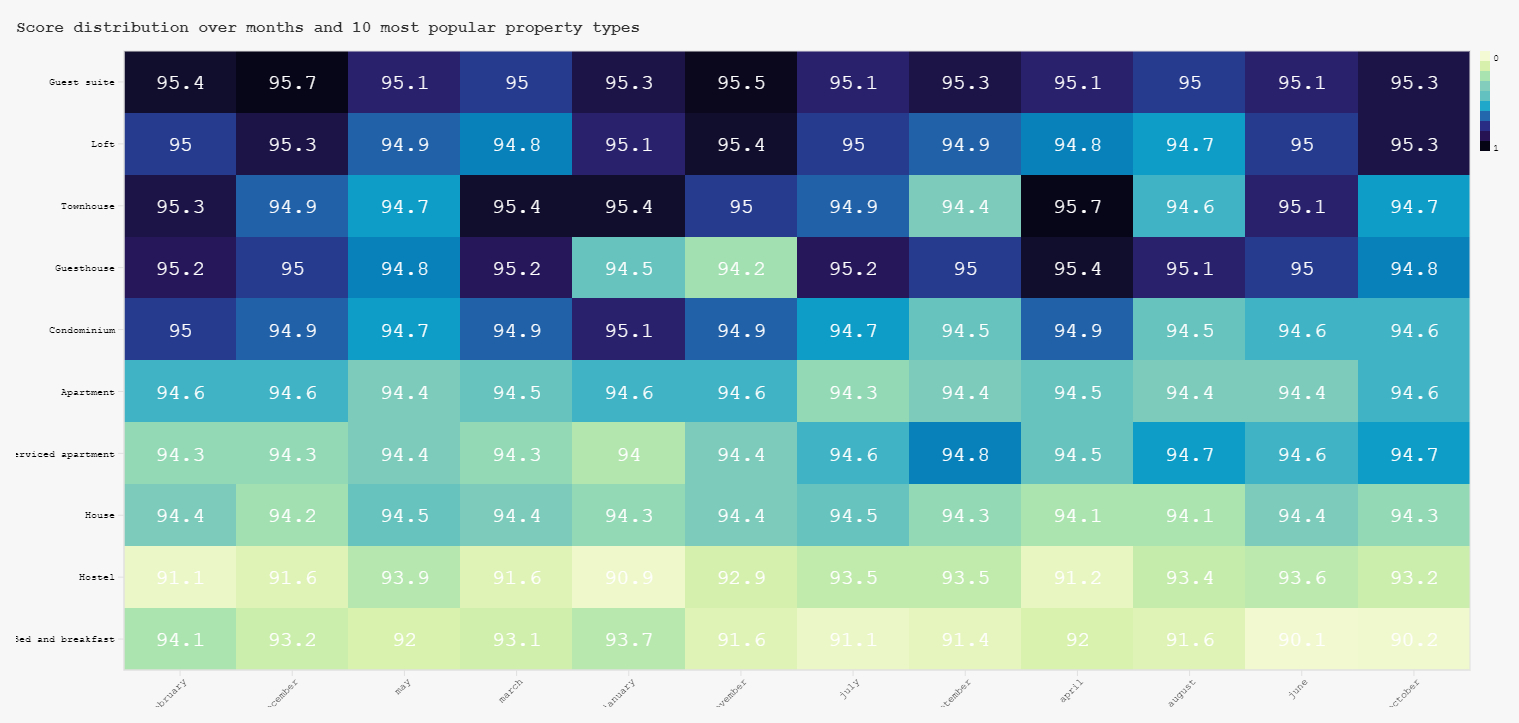
\includegraphics[width=1\textwidth]{images/q4_1.jpg}
    \caption{Score distribution over months and 10 most popular property types}\label{fig:figureq5}
\end{figure}

\vspace{1em}
\begin{figure}[H]
    \centering
    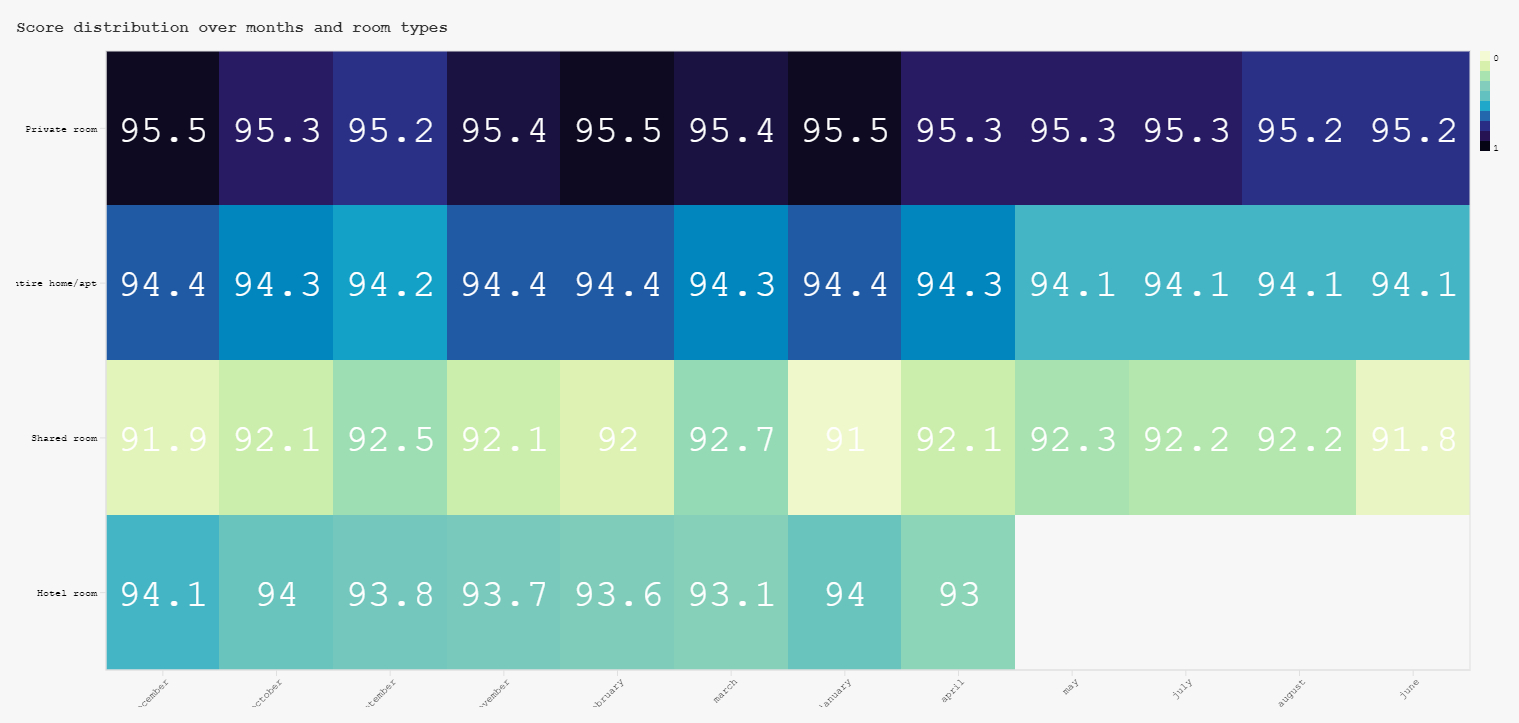
\includegraphics[width=1\textwidth]{images/q4_2.jpg}
    \caption{Score distribution over months and room types}\label{fig:figureq6}
\end{figure}

\vspace{1em}
\begin{figure}[H]
    \centering
    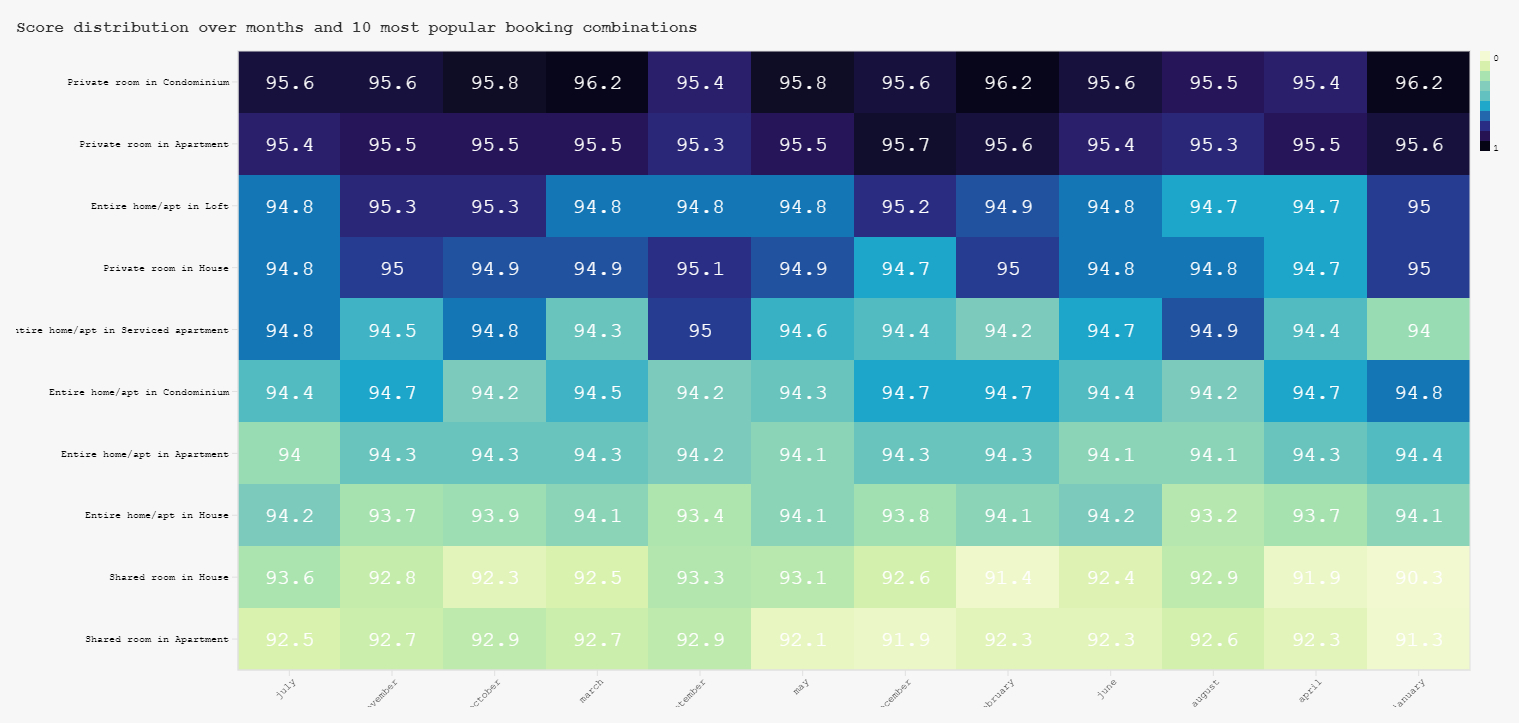
\includegraphics[width=1\textwidth]{images/q4_3.jpg}
    \caption{Score distribution over months and 10 most popular booking combinations}\label{fig:figureq7}
\end{figure}

\vspace{1em}
\begin{figure}[H]
    \centering
    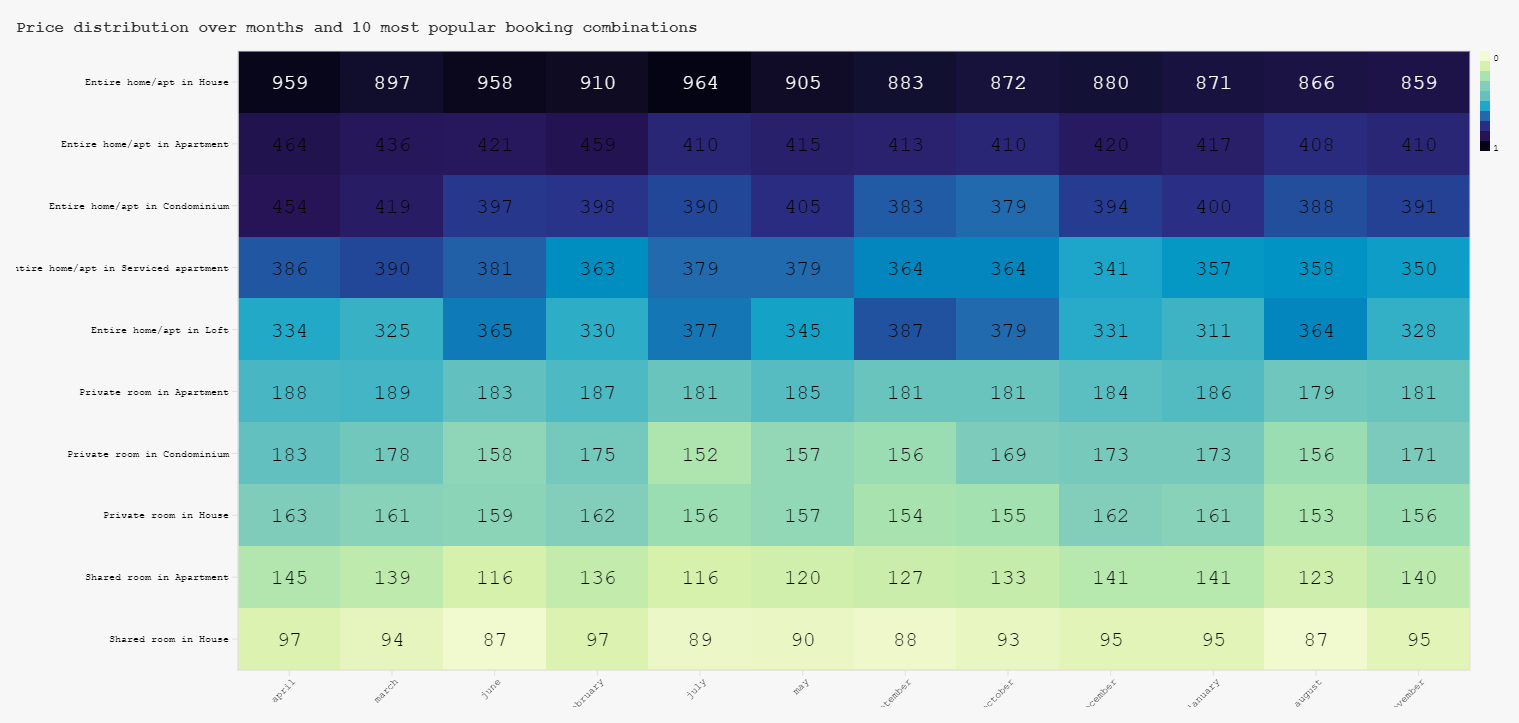
\includegraphics[width=1\textwidth]{images/q4_4.jpg}
    \caption{Price distribution over months and 10 most popular booking combinations}\label{fig:figureq8}
\end{figure}


\subsubsection*{5. Host Responsiveness and its Impact on Guest Experience }

This analysis investigates how host responsiveness (response time and response rate) relates to guest satisfaction and pricing. Buckets for both price and response rate allow easier pattern recognition.

\vspace{0.5em}
\paragraph{Key insights}
\begin{itemize}
    \item Faster is Generally Better: Across most price categories (except premium 2000\$+ segment), faster host response times correlate with higher review scores. Scores tend to decrease as response time lengthens to `within a day' and further to `a few days or more'.
    \item Unusual Premium Pattern for Response Time: The 2000\$ category shows a slightly unusual pattern: the `a few days or more' category surprisingly has the highest average score. This could be due to a smaller sample size in this specific high-end segment for slow responders, or perhaps the hosts of this segment just do not communicate with the most of customers, preferring small number of elites.
    \item Higher Response Rate Mean Higher Scores: This shows a quite strong and consistent positive correlation. The more consistently a host responds, the higher their review scores, almost regardless of the listing's price.
\end{itemize}

\vspace{1em}
\begin{figure}[H]
    \centering
    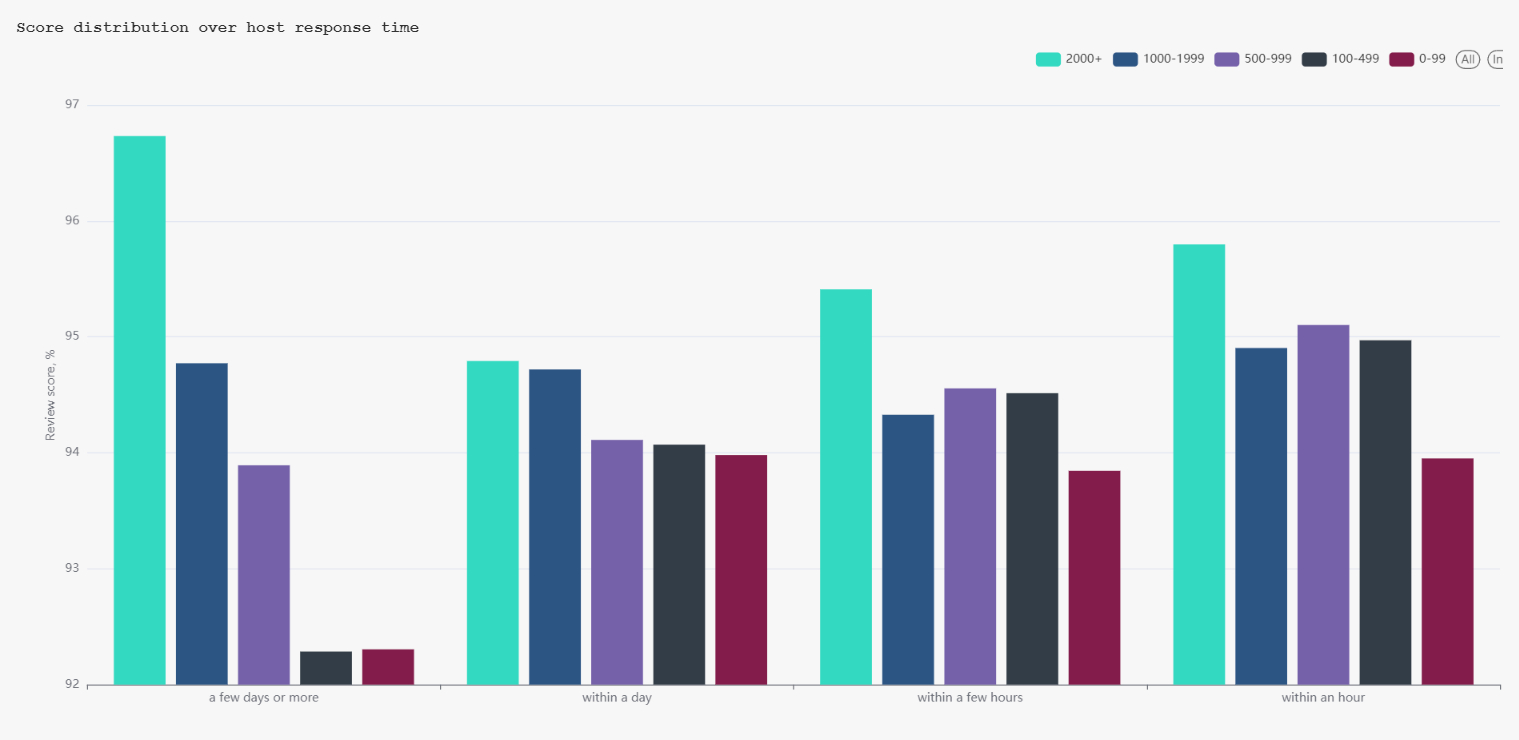
\includegraphics[width=1\textwidth]{images/q5_1.jpg}
    \caption{Score distribution over host response time}\label{fig:figureq9}
\end{figure}

\vspace{1em}
\begin{figure}[H]
    \centering
    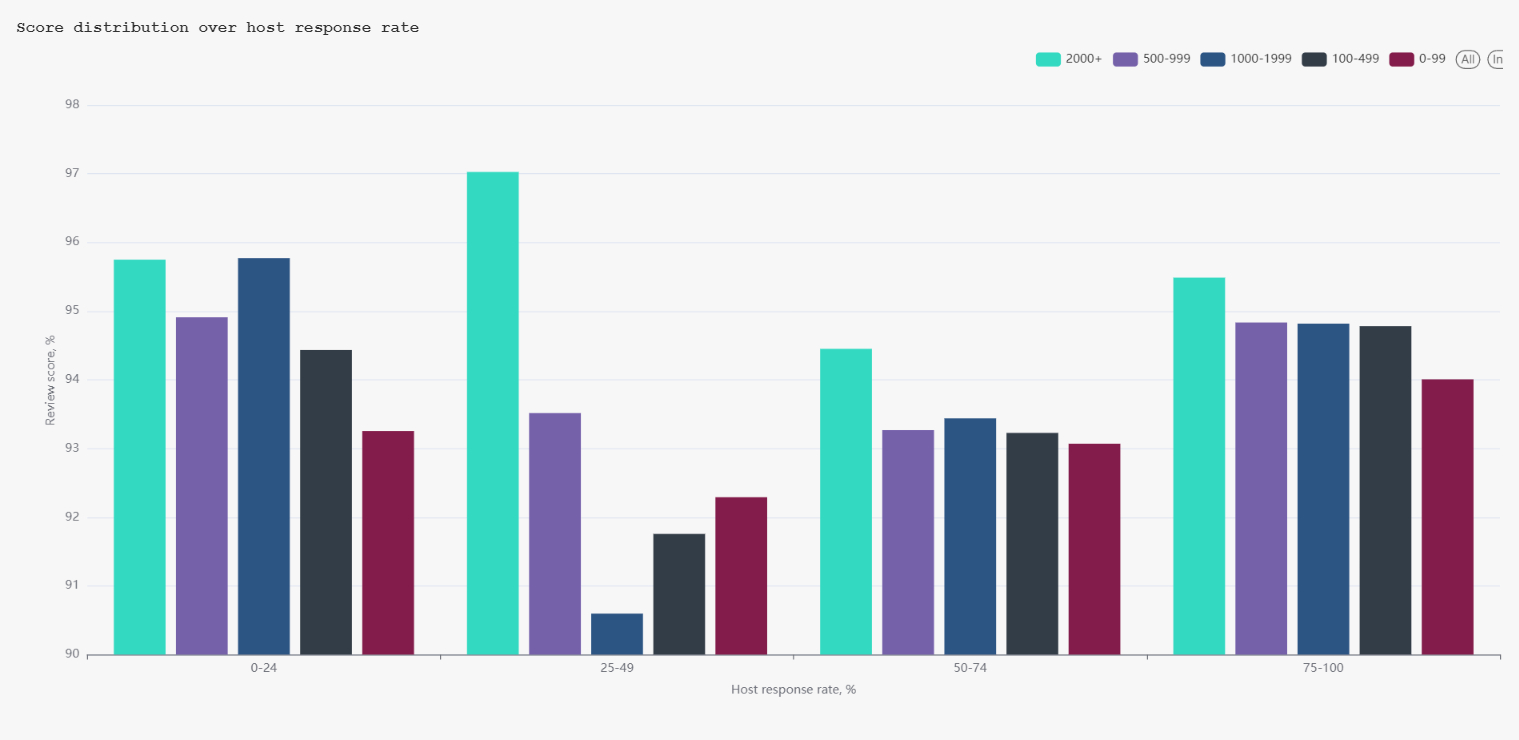
\includegraphics[width=1\textwidth]{images/q5_2.jpg}
    \caption{Score distribution over host response rate}\label{fig:figureq10}
\end{figure}


\subsubsection*{6. Geospatial Distribution of High-Value and Highly-Rated Neighborhoods}

In this query, we geolocate listings and mark those belonging to:
\begin{itemize}
    \item Concentration of High Scores and Prices: Both the `Mean score map' and `Mean price map' show clear concentrations of higher values in specific areas, predominantly along the southern coastal strip of Rio de Janeiro (likely encompassing famous touristic areas). There's a strong visual similarity in the distribution patterns of high scores and high prices.
    \item Overlap of Top Price and Top Score Neighborhoods: the overlap exists but is not strong. Most overlapping occurs in central regions of Rio de Janeiro, where both review scores and prices are high. The south-west part of the city is high-priced and (relatively) low-scoring, whilenorth past is, vice versa, low-priced but very high-scoring. So the key finding is that central neighborhoods `hidden-gems', so should have higher rating.
\end{itemize}

This is useful for mapping `premium' vs `well-rated' areas.

\vspace{0.5em}
\paragraph{Key insights}
\begin{itemize}
    \item Spatial clustering of high-value vs high-rating areas can inform geographic segmentation.
    \item Opportunity to identify luxury vs customer-favorite locations.
\end{itemize}

\vspace{1em}
\begin{figure}[H]
    \centering
    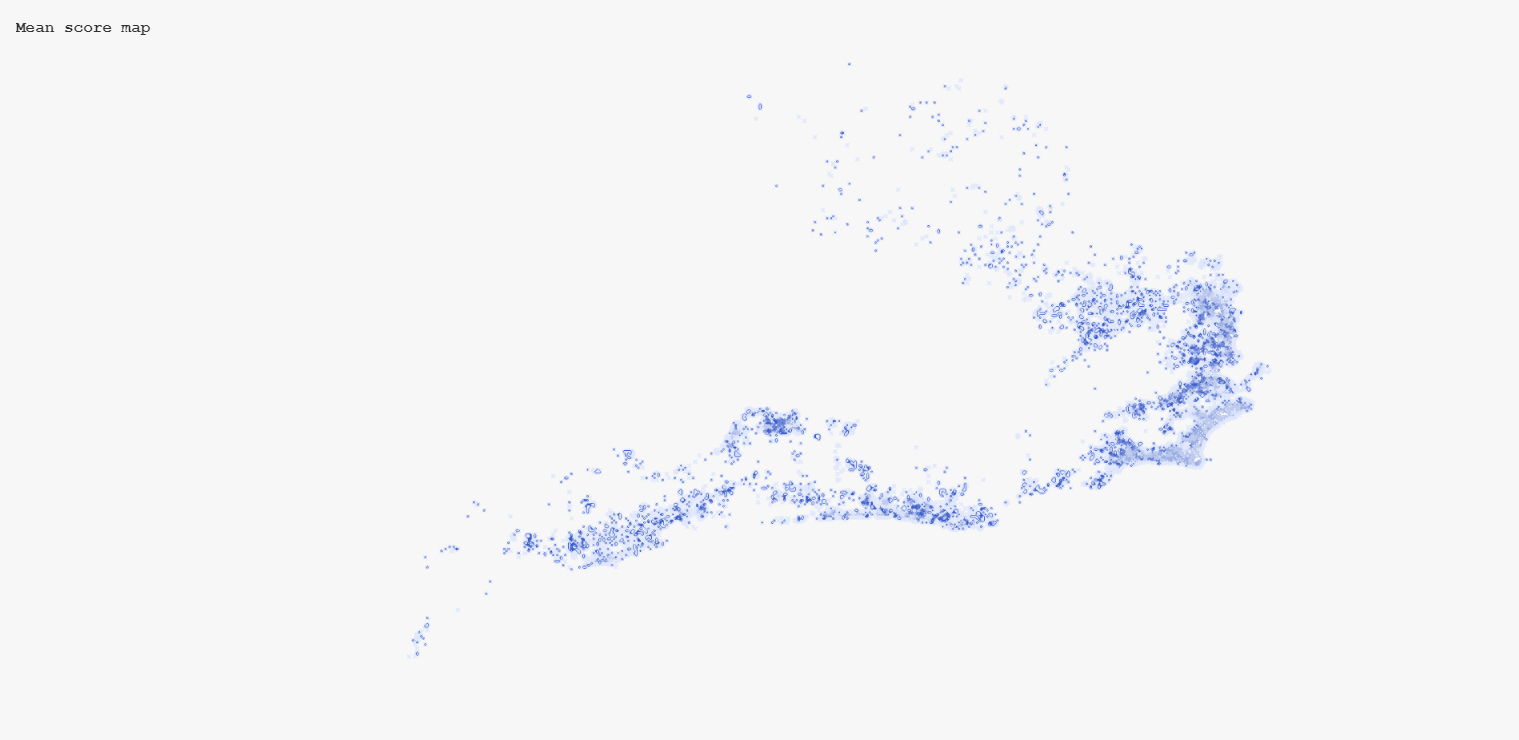
\includegraphics[width=1\textwidth]{images/q6_1.jpg}
    \caption{Mean score map}\label{fig:figureq11}
\end{figure}

\vspace{1em}
\begin{figure}[H]
    \centering
    
\includegraphics[width=1\textwidth]{images/q6_2.jpg}
    \caption{Mean price map}\label{fig:figureq12}
\end{figure}

\vspace{1em}
\begin{figure}[H]
    \centering
    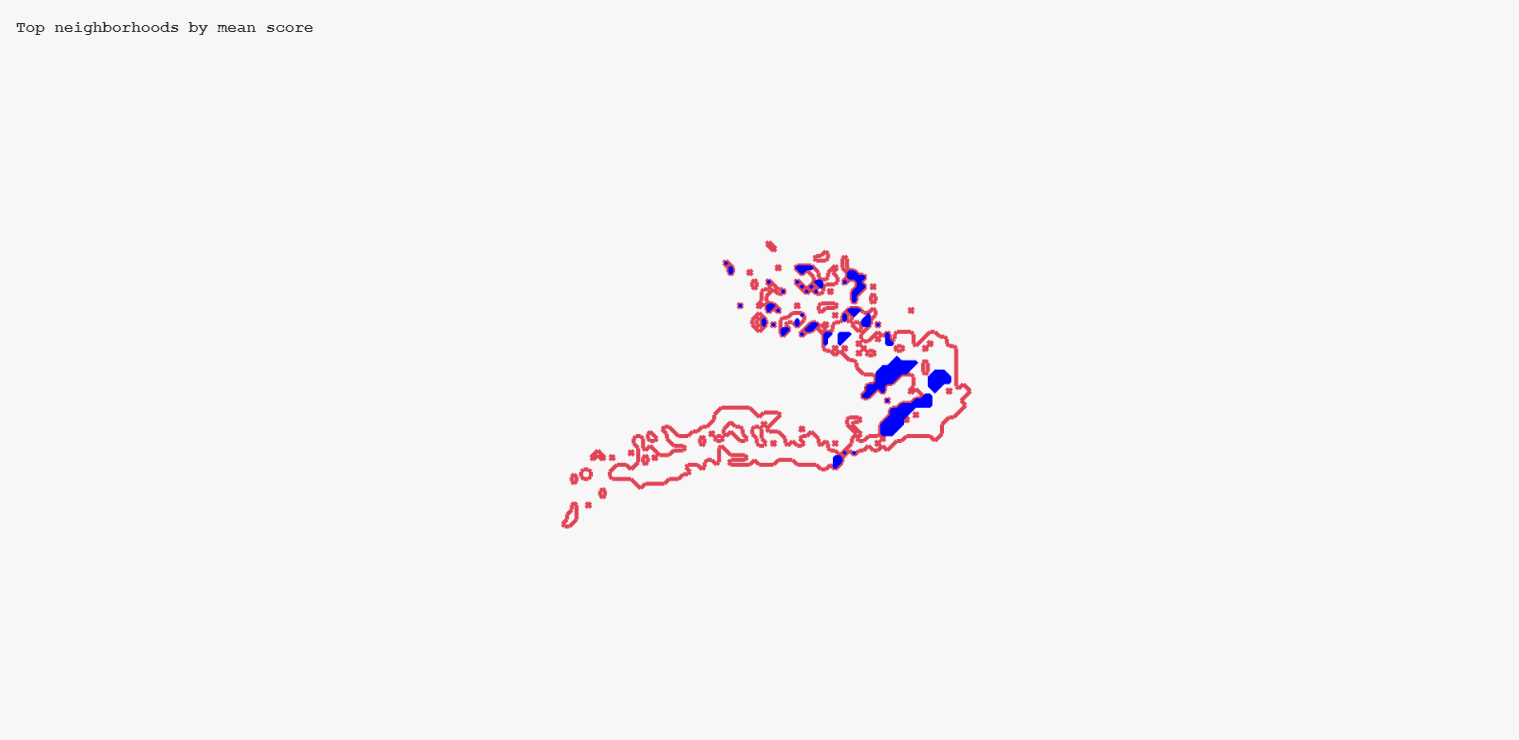
\includegraphics[width=1\textwidth]{images/q6_3.jpg}
    \caption{Top neighborhoods by mean price}\label{fig:figureq13}
\end{figure}

\vspace{1em}
\begin{figure}[H]
    \centering
    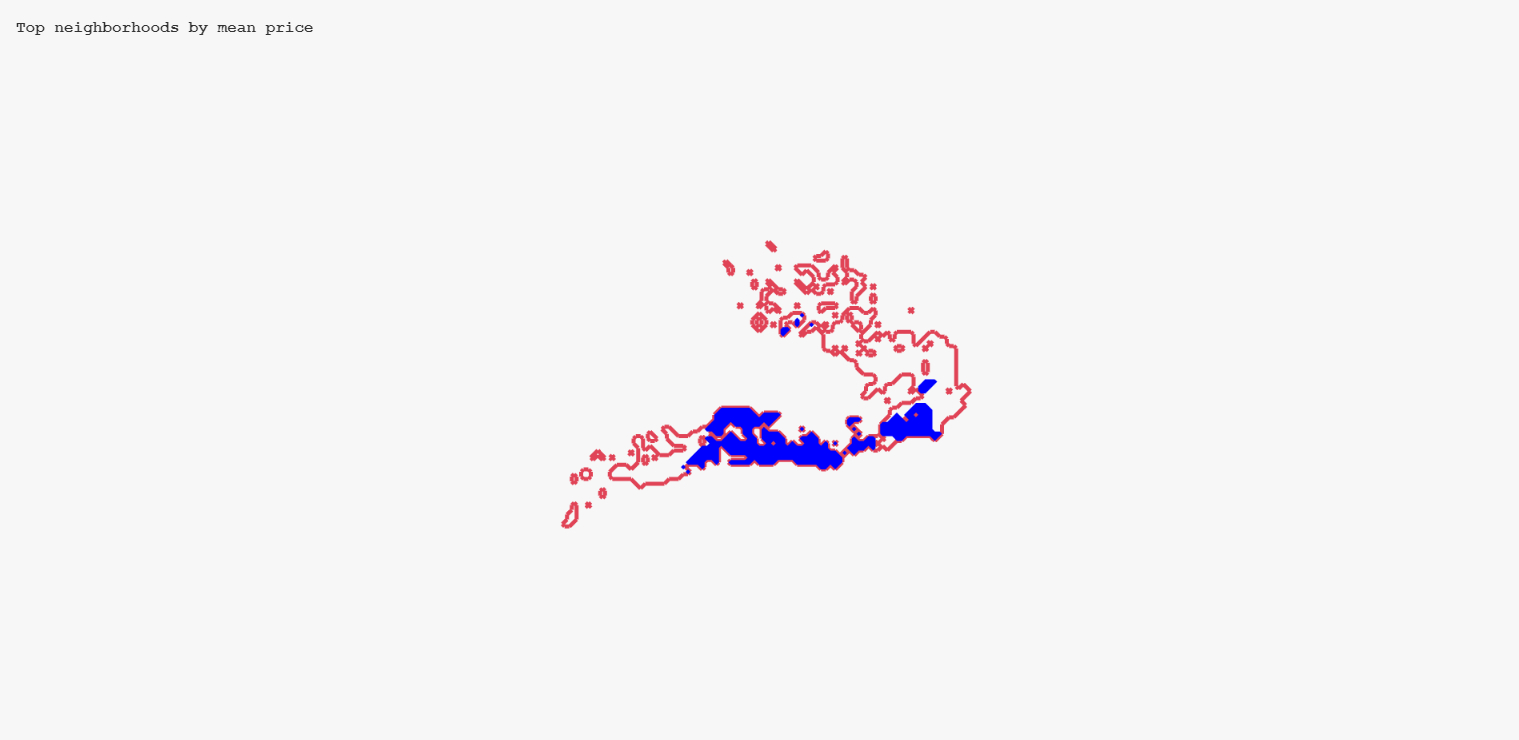
\includegraphics[width=1\textwidth]{images/q6_4.jpg}
    \caption{Top neighborhoods by mean score}\label{fig:figureq14}
\end{figure}

\subsubsection*{7. Amenity Combinations and Their Influence on Price and Ratings}

This final analysis categorizes listings based on presence of key amenities: Wi-Fi, air conditioning, hot water, and refrigerator. We assess how different combinations affect price and satisfaction.

\vspace{0.5em}
\paragraph{Key insights}
\begin{itemize}
    \item WiFi is Critical: Listings with WiFi, especially in combination with other key amenities like AC and a fridge, dominate the high scores. Even wifi\_only generally outperforms listings with only AC, only a fridge, or only hot water.
    \item Air Conditioning (AC) is Highly Valued: Particularly when paired with WiFi. Given climate of Rio de Janeiro, this is unsurprising.
    \item Hot Water is an Expectation: Its presence in `all\_amenities' contributes to high scores, but hotwater\_only scores poorly. This suggests it's a baseline necessity rather than a feature that elevates a listing if other desirable amenities are absent.
    \item Seasonal Impact: There are minor monthly fluctuations for most combinations, but the overall ranking of amenity packages by score remains largely the same throughout the year. For example, the need for AC might be perceived as slightly less critical in cooler months, but listings with wifi\_ac still outperform those with just wifi\_only.
\end{itemize}

\vspace{1em}
\begin{figure}[H]
    \centering
    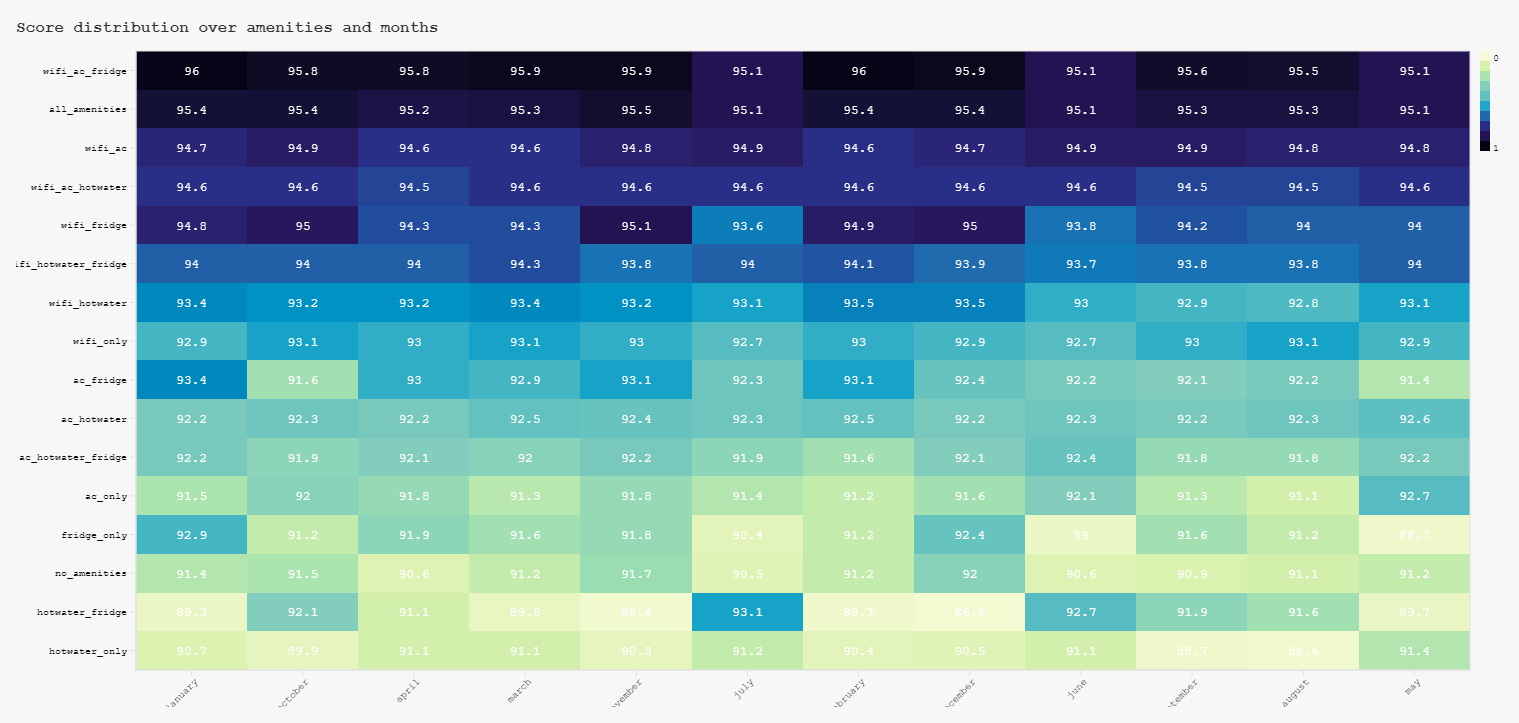
\includegraphics[width=0.8\textwidth]{images/q7_1.jpg}
    \caption{Score distribution over amenities and months}\label{fig:figureq15}
\end{figure}


Further transformations and detailed exploration will build on these findings to enhance data quality and modeling performance.



\subsection{Data quality}\label{sec:dataQuality}
An assessment of data quality revealed several issues:

\begin{itemize}
    \item All rows in our dataset have one or more null value, which is why we limit ourselves to certain features subset, that would be reviled in the next section.
    \item Several columns have problematic format. For example, column `amenities' is presented in format \{attr1, attr2, \ldots \}, which requires additional efforts for formatting.
    \item Almost half of our dataset misses our target feature `review\_scores\_rating' (385K out of 784K).
\end{itemize}

These issues will be addressed through data cleaning steps during the Data Preparation phase. Despite these inconsistencies, the dataset is overall of acceptable quality for modeling purposes.
